%% $RCSfile: proj_report_outline.tex,v $
%% $Revision: 1.3 $
%% $Date: 2016/06/10 03:41:54 $
%% $Author: kevin $

\documentclass[11pt
              , a4paper
              , twoside
              , openright
              ]{report}


\usepackage{float} % lets you have non-floating floats

\usepackage{url} % for typesetting urls
\usepackage{graphicx}
\usepackage{blindtext}
\usepackage{amsthm}
\usepackage[ruled,vlined]{algorithm2e}
\usepackage[T1]{fontenc}
\usepackage{float}
\usepackage[nottoc,numbib]{tocbibind}
\usepackage{amsmath}
\usepackage{mathtools}
\usepackage{cases}
\usepackage{multirow}
\usepackage{subcaption}
\usepackage{mdframed} % Add easy frames to paragraphs
\usepackage{lipsum} % For dummy text
\usepackage{xcolor}
\usepackage{xparse} % Add support for \NewDocumentEnvironment
\definecolor{graylight}{cmyk}{.30,0,0,.67} % define color using xcolor syntax
\theoremstyle{definition}
\newtheorem{exmp}{Example}[section]
%
%  We don't want figures to float so we define
%
\newfloat{fig}{thp}{lof}[chapter]
\floatname{fig}{Figure}

%% These are standard LaTeX definitions for the document
%%                            
\title{Using Graph Databases for Automatic QoS-Aware Web Service Composition}
\author{Zhaojiang Zhang}

%\subject{Software Engineering}

%% This file can be used for creating a wide range of reports
%%  across various Schools
%%
%% Set up some things, mostly for the front page, for your specific document
%
% Current options are:
% [ecs|msor|sms]          Which school you are in.
%                         (msor option retained for reproducing old data)
% [bschonscomp|mcompsci]  Which degree you are doing
%                          You can also specify any other degree by name
%                          (see below)
% [font|image]            Use a font or an image for the VUW logo
%                          The font option will only work on ECS systems
%
\usepackage[image,ecs]{vuwproject}

% You should specifiy your supervisor here with
\supervisor{Hui Ma}
% use \supervisors if there is more than one supervisor

% Unless you've used the bschonscomp or mcompsci
%  options above use
\otherdegree{Bachelor of (Software) Engineering}
% here to specify degree

% Comment this out if you want the date printed.
\date{}
\newmdenv[ % Define mdframe settings and store as leftrule
  linecolor=graylight,
  topline=false,
  bottomline=false,
  rightline=false,
  skipabove=\topsep,
  skipbelow=\topsep
]{leftrule}

\NewDocumentEnvironment{example}{O{\textbf{Example:}}} % Define example environment
{\begin{leftrule}\noindent\textcolor{graylight}{#1}\par}
{\end{leftrule}}
\begin{document}

% Make the page numbering roman, until after the contents, etc.
\frontmatter


%%%%%%%%%%%%%%%%%%%%%%%%%%%%%%%%%%%%%%%%%%%%%%%%%%%%%%%

%%%%%%%%%%%%%%%%%%%%%%%%%%%%%%%%%%%%%%%%%%%%%%%%%%%%%%%

\begin{abstract}
A Web service is a software component that takes input data and produces output data. With the rapid development of computer network technology, the demand for online services has grown, as has users' expectation that the quality of online services will meet their demands. To complete complex tasks, multiple Web services must be used, and it is necessary to combine, or compose these Web services to provide functions needed by users. The objective of service composition is to find a composite service that meets certain functional requirements and provides the best quality of service (\emph{QoS}), in a challenging environment where the number of available services is rapidly increasing. Existing approaches to service composition suffer from the drawback of requiring excessive computation in in order to find a service composition that meets functional requirements. We propose an automated QoS-Aware Web service composition approach using graph databases to store information taken from service repositories. We will show that our proposed approach can efficiently find service composition solutions.\end{abstract}

%%%%%%%%%%%%%%%%%%%%%%%%%%%%%%%%%%%%%%%%%%%%%%%%%%%%%%%

\maketitle
%\renewcommand{\baselinestretch}{1.27} 

\chapter*{Acknowledgments}\label{C:ack} 

I would like to express my deepest appreciation to all those who supported me in completing this report. I wish to pass on special gratitude to my supervisor, Dr Hui Ma, who provided abundant help, stimulating suggestions, and much needed support, encouragement and guidance during the project and preparation of this report. Special thanks to Alexandre Sawczuk da Silva, who helped me greatly with suggestions and ideas during the project. I also wish to express my gratitude to my and my wife's families for their kind cooperation, encouragement and support which enabled me to complete this project. 


\tableofcontents

% we want a list of the figures we defined
%\listof{fig}{Figures}

%%%%%%%%%%%%%%%%%%%%%%%%%%%%%%%%%%%%%%%%%%%%%%%%%%%%%%%

\mainmatter

%%%%%%%%%%%%%%%%%%%%%%%%%%%%%%%%%%%%%%%%%%%%%%%%%%%%%%%

% individual chapters included here
\chapter{Introduction}\label{C:intro}
Service-Oriented Architecture (SOA) \cite{1} is an architectural style for building software applications which uses services available in a network. SOA is realised through a standards-based technology called Web services, which allows coupling between Web services, so they can be reused. A Web service is a self-contained unit with limited functionality, that takes input data and produces output data \cite{27}. To provide value-added functions, it is necessary to compose Web services to provide powerful service functions. The result of such composition is to take a set of input data provided by the user and create a corresponding set of output data needed by a user.  

Currently there are three main approaches to Web service Composition. The first group of approaches includes several those which employ traditional methods such as Integer Linear Programming (ILP) \cite{7} to solve the problem of Web service composition. These approaches are lack of scalability and are no longer efficient since the number of Web services is increasing extraordinarily quickly. The second group includes various Evolutionary Computing (EC) approaches, such as Genetic Algorithms (GA) \cite{8}, Genetic Programming(GP) \cite{14,2,9} and Particle Swarm Optimisation (PSO) \cite{10,19}. These approaches are slow, especially when checking the dependencies between the component services, a task which requires a substantial amount of resources. The third type is the graph based approach, such as \cite{13,5}. This approach stores graph dependencies in memory temporarily rather than saving them permanently on local storage.


\section{Aims and Objectives}
The aim of this project is to propose an efficient automated QoS-aware Web service composition approach using Graph Databases. Existing Web service composition approaches \cite{2, 4} do not permanently store Web service dependencies, which means that when running the composition algorithm for different tasks, the algorithm will keep Web service dependencies in memory. The problem with this is that when a new task needs to be carried out, it becomes necessary to regenerate its Web service dependencies. This is because different tasks have different enquire (input) and result (outputs) data, upon which Web service dependencies are based. In practice, this behaviour dramatically increases the cost of running the system, since Web service dependencies which need only be generated once may in fact be generated several times. Moreover, the existing approach requires the generation of a corresponding workflow after each composition has been established. This takes a substantial amount of time and slows down the entire process.


Graph databases store data and  \cite{6} between data as graphs. In this project we employ a graph database to store the dependencies between services in a service repository and our service composition approach is based on the use of these graph databases. This project aims to create a graph database-based approach that generates Web service solutions efficiently by reducing the composition costs involved in checking dependencies of services. 

To achieve the aim of the project, the project is conducted with the following objectives:
\begin{enumerate}
  \item To review existing works in literature on this topic.
  \item To use a graph database to model and store services and their dependencies within a service repository.
  \item To generate non-QoS-aware Web services compositions with no redundant services in the compositions.
  \item To select service compositions with the best QoS. 
  \item To conduct a full evaluation of our approach by comparing the performance of our proposed approach with one of the existing approaches.
\end{enumerate}



\section{Structure of Report} 
This remainder of the report is organised as follows: A background and literature review is presented in Chapter 2. Chapter 3 gives a description of our Graph database-based approach. Chapter 4 covers our evaluation to compare the performance of our approach with an existing approach.  The final section of this report presents our conclusions regarding our approach, and proposes possible future developments regarding our approach.



\chapter{Background and Literature Review}\label{C:ex}
\section{Background}
\subsection{\emph{QoS}-Aware Web Service Composition}

Web services \cite{24} are modular, distributed, self-contained, dynamic applications that are published on the Web in order to be available to users. They follow certain technical standards such as Simple Object Access Protocol (SOAP) \cite{24} for accessing Web services, Web Service Description Language (WSDL) \cite{24} for describing Web services, and Universal Description, Discovery and integration (UDDI) \cite{25} for describing, publishing, and finding web services. \par

Web Services can be called by internet software and can be reused over and over by many applications. In essence, a web service is any piece of software that makes itself available over the internet \cite{27}.\par
\begin{exmp}
If I post pictures on Flickr about various steps needed to build my house, I may wish to dynamically display certain pictures. However, the relevant images are not stored on my local storage, but on Flickr. In this case I can make a dynamic request to ask Flickr to provide me with an image, since Flickr provides such a Web service.
This is the example.
\end{exmp}

However, it is important to note that a single Web service may only provide limited functionality, which is not sufficient to respond to the user's request. In order to complete complex tasks, a range of Web services are required, and it is necessary to combine, or compose these Web services to provide new value-added and complex functionality \cite{28}. When a user's request cannot be fulfilled by any available web service then Web Service Composition is required to fulfill the user's request.\

Web service composition is the process of combining several Web services into a more complicated and powerful service. Since there is no uniform definition, different researchers have defined the Web service composition problem from different perspectives \cite{22,21,23,20}. In \cite{20}, from the point of view of business processes, Web service composition is regarded as the organic connection of services according to certain business rules, so that companies can cooperate with each other to reach certain established business goals. In \cite{21}, from the perspective of application integration, Web service composition is the process of seamlessly integrating heterogeneous information systems and software from different enterprises, eliminating information silos and forming interconnected software consortia. In \cite{22}, from the point of view of problem solving, Web service composition is considered to be a way to achieve user-specific objectives, and a combination service satisfying this goal is found in a given set of services. In \cite{23}, from the point of view of task planning, service composition is a process of decomposing a large task into several subtasks, and breaking down these subtasks into even more smaller subtasks.\par

This project considers Web service composition to be the process of synthesizing several Web services when a single Web service can not meet a user's requirements, so as to form a large-scale composite service with internal process logic.\par

Nowadays, a large number of Web services on the Internet provide the same or overlapping functionality but present different non-functional characteristics. These non-functional characteristics are called Quality of Service (\emph{QoS}) properties, such as response time, execution cost, availability, reliability etc. Each of those properties are described in detail in the next section. Because \emph{QoS} properties have become the most commonly used set of characteristics for measuring the quality of Web services, meeting global \emph{QoS} requirements while fulfilling various functional requirements is referred to as \emph{\emph{QoS}-aware Web service composition} \cite{26,28}.


\subsection{\emph{QoS} Properties}
Quality of service (\emph{QoS}) is one of the important factors to consider when composing services. It defines the non-functional requirements of a service, such as response time, execution cost, availability, reliability etc. Good quality of service means achieving certain \emph{QoS} goals which are termed \emph{QoS} values or \emph{QoS} properties. These \emph{QoS} properties indicate whether a Web service is reliable, trustworthy or efficiency. Their significance stems from the fact that a Web service may be functionally capable of performing a given task, but might not be reliable or efficient enough to achieve users' satisfaction. Web services are usually rated using multiple \emph{QoS} values, each value representing an aspect, or \emph{QoS} property, of the Web service. \emph{QoS} properties are the most commonly used characteristics for measuring the quality of Web services and even composite services, as they indicate whether a service is capable of meeting users' expectations.\par

To model the performance of service compositions we considered four \emph{QoS} attributes: \emph{availability, reliability, execution cost} and \emph{response time}. We chose these because they are commonly used in this field \cite{15,14,16,4}. According to \cite{11,4,18}, the four above-mentioned \emph{QoS} properties are defined as follows:\par

\emph{Execution Cost} is the amount of money that a service requester has to pay for using the Web service. The global \emph{execution cost} \emph{$C_t$} of a composite set of services can be treated as the sum of the execution costs of all the operations invoked by the services \emph{s} used. 
\begin{equation}
C_t = \sum_{i=1}^{|s|} C_i
\end{equation}
$$\text{Where} |s| \text{is the number of services in the composition.}$$


The \emph{response time} of a single task is the time which elapses between sending a task request and receiving a response. Web service composition allows services to execute in parallel. Thus, when considering a step where two tasks execute in parallel, the path with the longest \emph{response time} is chosen to calculate the time taken for that step.\par

\begin{equation}
T_i = \left\{
\begin{split}
    \sum_{i=1}^{|s|} T_i      & \quad \text{if sequential pattern  } \\
    \max_{i=1}^{|s|} T_i      & \quad \text{if paraller pattern } \\
\end{split}\right. 
\end{equation}

\emph{Availability} is defined as the ratio of (1) the time during which a service is ready for use and (2) the time during which the Web service exists. The global availability \emph{$A_t$} of a composite Web services can be computed as the product of the local availabilities of the Web services \emph{s} used in the service composition.
\begin{equation}
 A_t = \prod_{i=1}^{|s|} A_i
\end{equation}

\emph{Reliability} is the how reliable message delivery is to the Web service within the maximum permitted time frame. Global \emph{reliability} \emph{$R_t$} can be calculated as the product of the local reliabilities of the Web services \emph{s} used in the service composition.
\begin{equation}
 R_t = \prod_{i=1}^{|s|} R_i
\end{equation}


\begin{figure}[H]
\includegraphics[width=9cm]{Figure2-1ExampleWebServiceComposition.pdf}
\centering
\caption{Example Web service composition}
\end{figure} 

\begin{exmp}
For example, for the service composition depicted in Figure 2.1, we can calculate the \emph{QoS} of the composition service using the above formulas as follows:
\setlength{\textfloatsep}{20pt}% Remove \textfloatsep

\setlength{\textfloatsep}{20pt}% Remove \textfloatsep
\emph{Execution cost}\par
The total \emph{execution cost} of the composite service can be calculated as: 
$$C_t = Cost(S_1) + Cost(S_2) + Cost(S_3) + Cost(S_4)$$
\setlength{\textfloatsep}{20pt}% Remove \textfloatsep

\setlength{\textfloatsep}{20pt}% Remove \textfloatsep
\emph{Response time}\par
In calculating \emph{response time}, it must be noted that, as shown in Figure 2.1, services $S_{2}$ and $S_{3}$ can be executed in parallel. The \emph{response time} depends on $S_{2}$ and $S_{3}$'s local \emph{QoS} duration property values. If $S_{2}$'s \emph{QoS} duration property value is greater than $S_{3}$'s \emph{QoS} duration property value, then the overall \emph{response time} of the composite service can be computed as the sum of all three service nodes $S_{1}$, $S_{2}$ and $S_{4}$'s local \emph{QoS} duration property values.\par  
$$T_t = Time(S_1) + Time(S_2) + Time(S_4)$$          
\setlength{\textfloatsep}{20pt}% Remove \textfloatsep

\setlength{\textfloatsep}{20pt}% Remove \textfloatsep
\emph{Availability}\par

The \emph{availability} of the composite service, can be computed as:
$$A_t = Availability(S_{1}) \times Availability(S_{3}) \times  Availability(S_{2}) \times Availability(S_{4}) $$
\setlength{\textfloatsep}{20pt}% Remove \textfloatsep

\setlength{\textfloatsep}{20pt}% Remove \textfloatsep
\emph{Reliability}\par
The \emph{reliability} of the composite service in Figure 2.1, 
can be computed as:
  $$R_t = Reliability(S_{1}) \times Reliability(S_{3}) \times Reliability(S_{2}) \times Reliability(S_{4})$$

\setlength{\textfloatsep}{20pt}% Remove \textfloatsep

\end{exmp}

\subsection {\emph{QoS}-Aware Fitness Functions} \label{fitnessFunction}

To evaluate the quality of a Web service composition we need a suitable fitness function. A fitness value can be used to reflect the global quality of service of a service composition. Following the common practice  \cite{19,14,4} used in multi-criteria optimization problems, we normalize the values of each \emph{QoS} property and restrict them to the interval [0,1]. We choose the same objective function as the one used in \cite{19,4} for our approach. The fitness for candidate \emph{i} is defined as follows:
\begin{equation}
Objective_{i}=(w_{1} \times A_{i}) + (w_{2} \times R_{i}) + (w_{3} \times T_{i}) + (w_{4} \times C_{i})
\end{equation}
\noindent
where \emph{A$_{i}$}, \emph{R$_{i}$}, \emph{T$_{i}$} and  \emph{C$_{i}$} denote the normalized availability, reliability,  execution cost and  execution time of candidate \emph{i}, and weights \emph{w} are real positive numbers where $w_{1} + w_{2} + w_{3} + w_{4} = 1$. The value of weights assigned by the user to the objective function represents the importance of the different \emph{QoS} properties for the Web service composition. \par

To achieve normalization we identify the minimum and maximum values of all the composition solutions discovered so far. We then use those values to normalize the \emph{QoS} properties according to the following formula \cite{4}:
\begin{equation}
A_i = \left\{
\begin{split}
    \frac{A_i - A_{min}}{A_{max} - A_{min}}      & \quad \text{if  } A_{max} - A_{min} \neq 0\\
    1  & \quad \text{if  } A_{max} - A_{min} = 0\\
\end{split}\right. 
\end{equation}

\begin{equation}
R_i = \left\{
\begin{split}
   \frac{R_i - R_{min}}{R_{max} - R_{min}}      & \quad \text{if  } R_{max} - R_{min} \neq 0\\
    1  & \quad \text{if  } R_{max} - R_{min} = 0\\
\end{split}\right. 
\end{equation}

\begin{equation}
T_i = \left\{
\begin{split}
    \frac{T_{max} - T_i}{T_{max} - T_{min}}      & \quad \text{if  } T_{max} - T_{min} \neq 0\\
    1  & \quad \text{if  } T_{max} - T_{min} = 0\\
\end{split}\right. 
\end{equation}

\begin{equation}
C_i = \left\{
\begin{split}
     \frac{C_{max} - C_i}{C_{max} - C_{min}}      & \quad \text{if  } C_{max} - C_{min} \neq 0\\
    1  & \quad \text{if  } C_{max} - C_{min} = 0\\
\end{split}\right. 
\end{equation}

Normalized \emph{QoS} property values close to \emph{1} indicate better quality, while normalized values closer to \emph{0} indicate poorer quality. Finally, we use the normalized \emph{QoS} properties and weights to calculate the fitness of the individual candidates, where the largest fitness value will be chose as the best Web service composition out of that set of candidates. 

\subsection{Graph Database and Neo4j}
A graph database is a type of \emph{NoSQL} database, which uses graph theory to store, map and query relationships. Graph databases contains \emph{nodes} and \emph{edges} components \cite{30}. They are widely used to model social networks and also used to solve real-world problems. \emph{Transportation} \cite{32}, \emph{protein-interaction} \cite{33} and even \emph{business networks} \cite{34} can naturally be modeled as graphs. Paper \cite{30} evaluates four current types of graph databases (\emph{Neo4j} \cite{6}, \emph{OrientDB} \cite{35}, \emph{Titan} \cite{36} and \emph{DEX} \cite{37})  from a performance point of view. The results show that the \emph{Neo4j} graph database gets the best performance with \emph{loading datasets}, \emph{finding the shortest path} and \emph{breadth-first exploration of nodes neighbourhood}. Good traversal performance reduces the time taken for Web service composition. \par

Because of its good performance, we employed a \emph{Neo4j} \cite{6} graph database for our project. We also chose it because it is suitable for representing connected and directed Web services and it allows for very fast retrieval, traversal and navigation of data. Our project used a \emph{Neo4j} graph database to store all services as \emph{nodes} and dependencies between the services as \emph{relationships} (edges). We gave all \emph{nodes} and \emph{relationships} their own individual properties. And for each data set we needed to create a graph database only once, after which we were able to use the database to solve various composition problems. \par

\section{Literature Review}
Over the past few years, Web services have become widely used. A large number of complex applications can be developed using compositions of existing services. Automatic Web service composition technology has become a major focus and challenge in building robust applications which make use of distributed services which provide various functions \cite{29}. Many approaches have been developed for Web service composition among which graph-based approach shows its promise in generating feasible composition solutions efficiently, but only a few of them use the concept of graph theory. In this section, we will present a brief overview of some graph-based techniques that deal with automatic Web service composition.
\par

Da Silva et al. presents in \cite{2} an evolutionary computation technique that performs fully automated Web service composition using graph representations for solutions. There are two steps. The first step is to initialise the population by employing a graph building algorithm based on the planning graph approach described in composition literature \cite{3}. The second step is to perform mutation and crossover operations on selected candidates, to generate a new set of candidates and evaluate the fitness of those candidates.\par
The drawback of the approach in \cite{2} is that the graph mutation space contains many invalid service compositions that either violate the constraints of service dependencies or deteriorate the overall performance. Another disadvantage is that the system only keeps the Web service dependencies in memory. With every new service request, this approach needs to regenerate all the dependencies again which incurs expensive computation costs. Furthermore, the cost of executing the graph building algorithm is high, since the graph building algorithm is employed twice, in two different processes, namely in the process of generating initial populations and the process of performing mutation and crossover operations.\par
Seyyed et al. \cite{5} uses a graph search algorithm to construct Web service compositions. This algorithm is based on input-output dependencies of Web services. In order to solve the service composition problem, the authors divide the process into two steps. The first step is to look for Web services which can potentially participate in the composition, and the second step is to find a corresponding composition. The graph building algorithm constructs edges between directly related Web services which have data dependencies between the inputs and outputs of these services. The main shortcoming of this approach is that semantic functions are not considered in the dependencies between input and output parameters. Thus there is no guarantee that a generated composite service will provide the precise functionality requested by the user.\par
The Web service composition approaches proposed by Da Silva et al. in \cite{2} and Seyyed et al. in \cite{5} also share a common drawback. They do not include quality of service in their approach. This means the resulting Web services may not perform tasks that meet a user's non-functional requirements.\par

Jing et al \cite{26} developed a relational-database approach to constructing Web service compositions. This approach overcomes a major limitation of most automated service composition methods \cite{2,5}, which was to store Web services and dependencies between them only in memory. This approach stores  Web services and dependencies between the Web services in a database instead of memory. The authors propose an algorithms that builds a path between services in the service repository. According to their method, each path has a PathID, and input and output values. After all paths have been generated, they are then stored in the database. To handle the task requests, a query must be sent to the database to find Web service composition paths which satisfy the request. The next step involves ranking and filtering the paths returned from the algorithms according to their \emph{QoS} value. The top rank will be the best composition for a given task. \par
One of the major drawbacks of the approach in \cite{26} is that it cannot efficiently handle a very large service repository. The proposed method is slow, as it preprocesses all the Web services in advance to generate paths between services which it stores in the database. However, if any service inputs or outputs have changed or any new Web services have been added, this will affect most of the paths stored in the database, since they are interconnected each other. In addition, many services offer identical or overlapping functionalities.\par
The result is that the number the paths in the database is enormous. And all the paths need to be processed in order to find the PathID and process the input and output of the each path in the related paths. So when creating web service compositions this greatly downgrades overall performance. The third drawback of the approach in \cite{26} is that it only considers the response time property when dealing with \emph{QoS}-aware Web service composition and does not consider execution cost, availability and reliability of the composition. This means the solution may not be the optimised solution.\par


As we have seen, existing graph-based \cite{5} and GP based \cite{2} approaches need to build a data dependency graph for each given task. However, database dependencies between services in a service repository remain stable for all service tasks. Therefore, once a service dependency graph is generated it should be stored, so it can be used for all service tasks. In this project, we propose to use a graph database to store the information related to services and dependencies of services of a service repository. Once a graph database has been created using information in the service repository, all the services and dependencies of the services are permanently stored on local storage, and a Graph database like Neo4j, which has built-in path-finding methods, is used. This is different to the relational-database approach in \cite{26}, where there is a need to generate all the paths between services and then store those paths in the database. With each new service task, our approach can utilise existing dependency information contained within graph database dependency graphs. Our approach also takes the quality of service (\emph{QoS}) into consideration by including \emph{QoS} properties with each edge between Web services.\par   
 
In summary, most current non-database-type automated Web service composition methods \cite{2,5} are in-memory methods, which means Web service composition results, details of services, and dependencies between services are stored locally in simple text format. This means the reusability of the solution is very low, as most information is not stored, especially in the case of service dependencies and services are not reusable after memory is cleared. The relational-database-based approach \cite{26} uses stored services with dependencies between services stored in the database as paths, but the performance of SQL queries on the large resulting database as well as database maintenance is very low.\par
\chapter{The Graph database-based Web Service Composition Approach}\label{C:wd}
This report focuses on the the use of graph databases to model and store a service repository, with dependencies between the Web services, and service compositions. Our graph based approach consists of four steps:\par
\begin{enumerate}
  \item Creating graph database for a web service repository: We use all available services in the service repository to create a graph database, with Web services as \emph{nodes} and dependencies between services as \emph{edges}.\par

  \item Generating a graph database for a given task: We selected all the services related to the given task inputs and outputs, then used related services to generate a graph database.\par

  \item Generating initial population of service composition solutions: We used the graph database we generated in step 2 and the algorithm we designed for this project to produce an initial population of service composition solutions.\par

  \item Selecting a service composition solution from the population with the best overall \emph{QoS}: We applied the fitness function to the initial population to find the solution with best overall \emph{QoS}.\par

\end{enumerate}
The overall design of our system is shown in Figure \ref{fig:process}, and the section following Figure \ref{fig:process} describes our design in detail.\par

\begin{figure}[H]
\includegraphics[width=10cm]{process.pdf}
\centering
\caption{Overall system design}
\label{fig:process} 
\end{figure} 

\section{Modelling of Web service Repository} \label{procesedGD}
\subsection {Web Service}
In this project we model a Web service as an entity which has a \emph{name}, and has a set of properties \emph{ID, QoS, inputs, outputs, inputServices, and outputServices}. The first step is to model service repositories, which contains a set of services, between which there are data dependencies. Data dependency refers to the relationships between services. Each service takes inputs, produce outputs, and has \emph{QoS}. In the following description of our approach we provide details of this model.\par
\subsection {Inputs and Outputs}
It is necessary to label each Web service for identification, and the different \emph{inputs} and  \emph{outputs} of each Web service should also be easily identifiable. In our approach we used a taxonomy tree to represent the relationships between the inputs and outputs of services. In the particular taxonomy tree we used, any two concepts \emph{A} and \emph{B} can be related to each other in one of four possible ways. The first scenario is that \emph{A} is a generalization of \emph{B}. The second scenario is that \emph{A} is a specialization of \emph{B}. The third scenario is that \emph{A} and \emph{B} are not related to each other. And the last scenario is that  \emph{A} equals \emph{B}. 
\newcommand{\quotes}[1]{``#1''}
\begin{example}
\noindent
The Web service \quotes{FindHotel} uses a single input parameter (cityName) represented by the concept of \quotes{CITY}, which belongs to the taxonomy tree. Therefore, \quotes{FindHotel} requires an instance of the concept \quotes{CITY}. The only output parameter (Hotel) is represented by an instance of the concept \quotes{Hotel} that also exists in the taxonomy tree. The \emph{inputs} and \emph{outputs} of each Web service are clearly defined in terms of concepts belonging to the specialized taxonomy tree.
\end{example}


\subsection {InputServices and OutputServices}
As shown in Figure \ref{fig:inputOutputServs}, within a Neo4j database, Web services are modelled as having a set of \emph{InputServices}, which is the set of Web services connected to the input side of the Web service, and  \emph{outputServices} which is the set of Web services connected to the output side of the service. The reason that we add these two properties is to make it easier to retrieve the connected Web services and also to reduce the cost of creating relationships between Web services. \par


\subsection {Web Service Dependencies}
Each relationship is a directed edge that connects the output of a Web service node to the input of another node according to already established dependencies stored in the taxonomy tree. Like Web service nodes, relationships also have properties. They have a \emph{from} node, a  \emph{to} node and direction. Relationships between Web service nodes are an essential part of a graph database. They allow us to find related Web services.  


\section {Generating a Graph Database for a Service Repository}

The previous section explained the components of the graph database we used in our approach to modelling a service repository in order to generate graph database.

There are three steps involved in generating our database. Firstly, preprocessing the service repository in order to find all the services' properties mentioned in section 3.1, and create a Web service object for each service in the service repository. Secondly, creation of the graph database Web service nodes using the web service objects we created in step 1. We accomplish this by assigning all the Web service objects' fields to graph database Web service node properties. Lastly, generation of graph database relationships based on the Web service nodes' input services and output services. The following sections will introduce the design in greater detail.   

\subsection{Preprocessing of the Service Repository}
In the previous section we explained the components of the graph database.  In this section we use a modelled service repository to generate a graph database.  Before generating a graph database, we need to preprocess the service repository by creating a Web service Object for each Web service from the service repository. Each Web service object contains all the properties as we mentioned in section 3.1. We then apply \emph{Algorithm 1} to find all the input services and output services for each taxonomy node. \emph{Algorithm 1} identifies all the input and output services for each Web service using a taxonomy tree. 




\setlength{\textfloatsep}{0pt}% Remove \textfloatsep
\begin{algorithm}[H]
 \SetKwInOut{Input}{Input}\SetKwInOut{Output}{Output}

 \SetKwFunction{connectNode}{connectNode}\SetKwFunction{findCands}{findCands}\SetKwFunction{removeDangling}{removeDangling}
 \LinesNumbered
 \SetNlSty{}{}{:}
  \Input{$taxonomyNodes$, $serviceNodes$}
 \Output{$taxonomyNodes$}
 $i \leftarrow 0$\;
 \While{$i < |taxonomyNodes|$}{\label{buildingLine}
 $tNode \leftarrow taxonomyNodes[i]$\;
 $tNode.parents \leftarrow findParentsNodes(tNode)$\;
 $tNode.children \leftarrow findChildrenNodes(tNode)$\; 
 $i \leftarrow i+1$\;
 }
  $i \leftarrow 0$\;
  \While{$i < | serviceNodes |$}{\label{buildingLine}
       $j \leftarrow 0$\;
       $outputs \leftarrow serviceNodes[i].outputs$\;
      \While{$j < |outputs|$}{\label{buildingLine}
        $tNode \leftarrow findTaxonomyNode(outputs[j])$\;
        $k \leftarrow 0$\;
        \While{$j < |tNode.parents|$}{\label{buildingLine}
          $tNode.parents \leftarrow tNode.parents\cup \{serviceNodes[i]\}$\;
          $k \leftarrow k+1$\;
        }
         $j \leftarrow j+1$\;
      }
       $j \leftarrow 0$\;
       $inputs \leftarrow serviceNodes[i].inputs$\;
       \While{$j < |inputs|$}{\label{buildingLine}
        $tNode \leftarrow findTaxonomyNode(inputs[j])$\;
        $k \leftarrow 0$\;
        \While{$j < |tNode.children|$}{\label{buildingLine}
          $tNode.children \leftarrow tNode.children\cup \{serviceNodes[i]\}$\;
          $k \leftarrow k+1$\;
        }
         $j \leftarrow j+1$\;
      }
 $i \leftarrow i+1$\;
 }
 \caption{\footnotesize Populates the taxonomy tree by associating services with the nodes in the tree.}
\label{generation}
\end{algorithm}
\setlength{\textfloatsep}{20pt}% Remove \textfloatsep


\begin{example}
\noindent
Service \emph{1} has inputs $I_1 = \{A\}$ and outputs $O_1 = \{B\}$, service \emph{2} has Inputs $I_2 = \{E\}$  and outputs $O_2 = \{B\}$, and service \emph{3} has Inputs $I_3 = \{B\}$  and outputs $O_3 = \{F\}$. \emph{Algorithm 1} searches services inputs and outputs of services \emph{1, 2} and \emph{3}. Each value in inputs and outputs is a node in the taxonomy tree, which we call a taxonomy node (\emph{tNode}). Each \emph{tNode} has input services (\emph{IS}) and output services (\emph{OS}) fields; then we add Web services into corresponding \emph{IS} or \emph{OS} field. Taxonomy is represented as a tree, and each \emph{tNode} can have a parent node or child node. For example, \quotes{CITY} \emph{tNode} may have parent node called \quotes{COUNTRY} and child node called \quotes{HOTEL}. When we add Web service into \emph{IS}, we also add a Web service into all the \emph{tNode}'s parent node's \emph{IS} field. The same applies to adding Web service into \emph{OS}, in which case we also add Web service into all the \emph{tNode}'s children node's \emph{OS} field. After we run \emph{algorithm 1}, we obtain $IS_A = \{service 1\}$, $OS_A = \{service 1, service 2, service 3\}$, $IS_B = \{service 1, service 3\}$, $OS_B = \{service 1, service 2\}$, $IS_E = \{service 1, service 3\}$, $OS_E = \{Null\}$, $IS_F = \{service 1\}$ and $OS_F = \{service 3\}$. This is shown in Figure \ref{fig:taxonomyTree}. \par

\end{example}

\begin{figure}[H]
\includegraphics[width = 10cm]{taxonomy-tree-example.pdf}
\centering
\caption{Taxonomy tree Example}
\label{fig:taxonomyTree} 
\end{figure} 

Then apply \emph{Algorithm 2} to assign input services and output services for each Web service object based on Web service object's \emph{inputs} and \emph{outputs}. \emph{Algorithm 2} goes through each input value in each Web service (\emph{WS}) in a service repository and finds a corresponding taxonomy node \emph{tNode} and then adds all the input services into the \emph{WS}'s \emph{InputServices} field. It also adds all the input services found in all parent taxonomy nodes into \emph{WS}'s \emph{IS} field. Additionally, it checks each output value in each \emph{WS} in a repository, and finds corresponding \emph{tNode} , adding all the output services into the \emph{WS}'s \emph{OS} field, and all the output services found in all parent taxonomy nodes into \emph{WS}'s \emph{OS} field.
\begin{example}
\noindent
After we run the \emph{algorithm 2}, we get: 
Service \emph{1}: $IS_1 = \{service 1, service 2, service 3\}$ and
 $OS_1 = \{service 1, service 3\}$,
Service \emph{2}: $IS_2 = \{Null\}$ and
$OS_2 = \{service 1, service 2\}$,
Service \emph{3}: $IS_3 = \{service 1, service 2\}$ and
 $OS_3 = \{service 1\}$, shown in Figure \ref{fig:inputOutputServs}.
\end{example}

\begin{figure}[H]
\includegraphics[width=10cm]{InputServicesAndOutServices.pdf}
\centering
\caption{Input services and out services}
\label{fig:inputOutputServs} 
\end{figure} 
\begin{algorithm}[H]
 \SetKwInOut{Input}{Input}\SetKwInOut{Output}{Output}
 \SetKwFunction{connectNode}{connectNode}\SetKwFunction{findCands}{findCands}\SetKwFunction{removeDangling}{removeDangling}
 \LinesNumbered
 \SetNlSty{}{}{:}
 \Input{$serviceNodes$}
 \Output{$serviceNodes$}
 $i \leftarrow 0$\;
 \While{$i < |serviceNodes|$}{\label{buildingLine}
   $sNode \leftarrow serviceNodes[i]$\;
   $sNode.inputServices \leftarrow \{\}$\;
   $sNode.outputServices \leftarrow \{\}$\;
   $j \leftarrow 0$\;
     \While{$j < |sNode.outputs|$}{\label{buildingLine}
        $tNode \leftarrow findTaxonomyNode(sNode.outputs[j])$\;
        $k \leftarrow 0$\;
      \While{$k < |tNode.outputServices|$}{\label{buildingLine}

          $sNode.outputServices \leftarrow sNode.outputServices\cup \{tNode.outputServices[k]\}$\;
          $k \leftarrow k+1$\;
      }
        $j \leftarrow j+1$\;
     }
      $j \leftarrow 0$\;
     \While{$j < |sNode.inputs|$}{\label{buildingLine}
        $tNode \leftarrow findTaxonomyNode(sNode.inputs[j])$\;
        $k \leftarrow 0$\;
      \While{$k < |tNode.inputServices|$}{\label{buildingLine}

          $sNode.inputServices \leftarrow sNode.inputServices\cup \{tNode.inputServices[k]\}$\;
          $k \leftarrow k+1$\;
      }
        $j \leftarrow j+1$\;
     }
   $i \leftarrow i+1$\;
 }
 
 \caption{\footnotesize Add correspondence input services and output services to each Web service.}
\label{generation}
\end{algorithm}
\setlength{\textfloatsep}{20pt}% Remove \textfloatsep
\subsection{Creation of Web Service Nodes}
Each Web service is a node in the graph database, and each node contains list of properties. In this section we will introduce how to create graph database Web service nodes using Web service objects we produced from service repository preprocessing section. We use graph database create node method to generate a new node and we use the setproperty method to assign properties to the node. We also create an index for each Web service node for querying the Web service node by its service name when needed. After service nodes have been created, all service nodes are stored in the graph database permanently.  Figure \ref{fig:noRelationships} is an example of a graph database - it shows the Web service nodes we created with no relationships created yet between the Web services. The data set used in this example is WSC 2008-01. All the nodes represent the Web services. 
\begin{figure}[H]
\includegraphics[width=10cm]{service-without-relationships.png}
\centering
\caption{Graph database without relationships (WSC 2008-01)}
\label{fig:noRelationships} 
\end{figure} 
\subsection {Creation of Web Service Dependencies}
In order to create Web service dependencies,  we need go through each Web service node in the graph database, find all the  \emph{input services} and  \emph{output services} and then use the  \emph{createRelationshipTo} method to create dependencies between the Web service nodes.  \emph{Algorithm 3} handles the process of creating relationships between Web services. It goes through each Web service node ( \emph{N}), and loops through the corresponding  \emph{inputServices} of each  \emph{N}, and then adds relationships between the Web services according to the sets of  \emph{inputServices}. \emph{Algorithm 3} handles the process of creating relationships between Web services. It goes through each Web service node \emph{N}, and loops through the corresponding \emph{inputServices} of each \emph{N}, and then adds relationships between the Web services according to the sets of \emph{inputServices}.

\setlength{\textfloatsep}{20pt}% Remove \textfloatsep
\begin{algorithm}[H]
 \SetKwInOut{Input}{Input}\SetKwInOut{Output}{Output}
 \SetKwFunction{connectNode}{connectNode}\SetKwFunction{findCands}{findCands}\SetKwFunction{removeDangling}{removeDangling}
 \LinesNumbered
 \SetNlSty{}{}{:}
 \Input{$GraphDatabaseWithNoRelationships$}
 \Output{$GraphDatabaseWithRelationships$}
 $i \leftarrow 0$\;
 \While{$i < |serviceNodes|$}{\label{buildingLine}
   $sNode \leftarrow serviceNodes[i]$\;
   $j \leftarrow 0$\;
     \While{$j < |sNode.inputServices|$}{\label{buildingLine}
      $inputSNode \leftarrow sNode.inputServices[j]$\;
      $relation \leftarrow inputSNode.createRelationshipTo(sNode)$\;
      $relation.setProperty("From" : inputsNode)$\;
      $relation.setProperty("To" : sNode)$\;
      $relation.setProperty("Outputs" : inputsNode.outputs)$\;
      $relation.setProperty("Direction" : incoming)$\;
        $j \leftarrow j+1$\;
      }
     $i \leftarrow i+1$\;
  }
 \caption{\footnotesize create relationships between Web services.}
\label{generation}
\end{algorithm}
\setlength{\textfloatsep}{20pt}% Remove \textfloatsep

\begin{example}
\noindent
Figure \ref{fig:beforeReduction} is an example of a graph database before reduction. The data set used in this example is WSC 2008 - 01, which contains is a total of 158 Web services. All the nodes represent the Web services and all the edges are the relationships between Web services. Once you click a node or an edge from the graph database, the properties of that node or edge appear at the bottom of the page. Figure \ref{fig:servProp} is an example of the properties that appear when you click the node Web service serv7231183. \par
\end{example}

\begin{figure}[H]
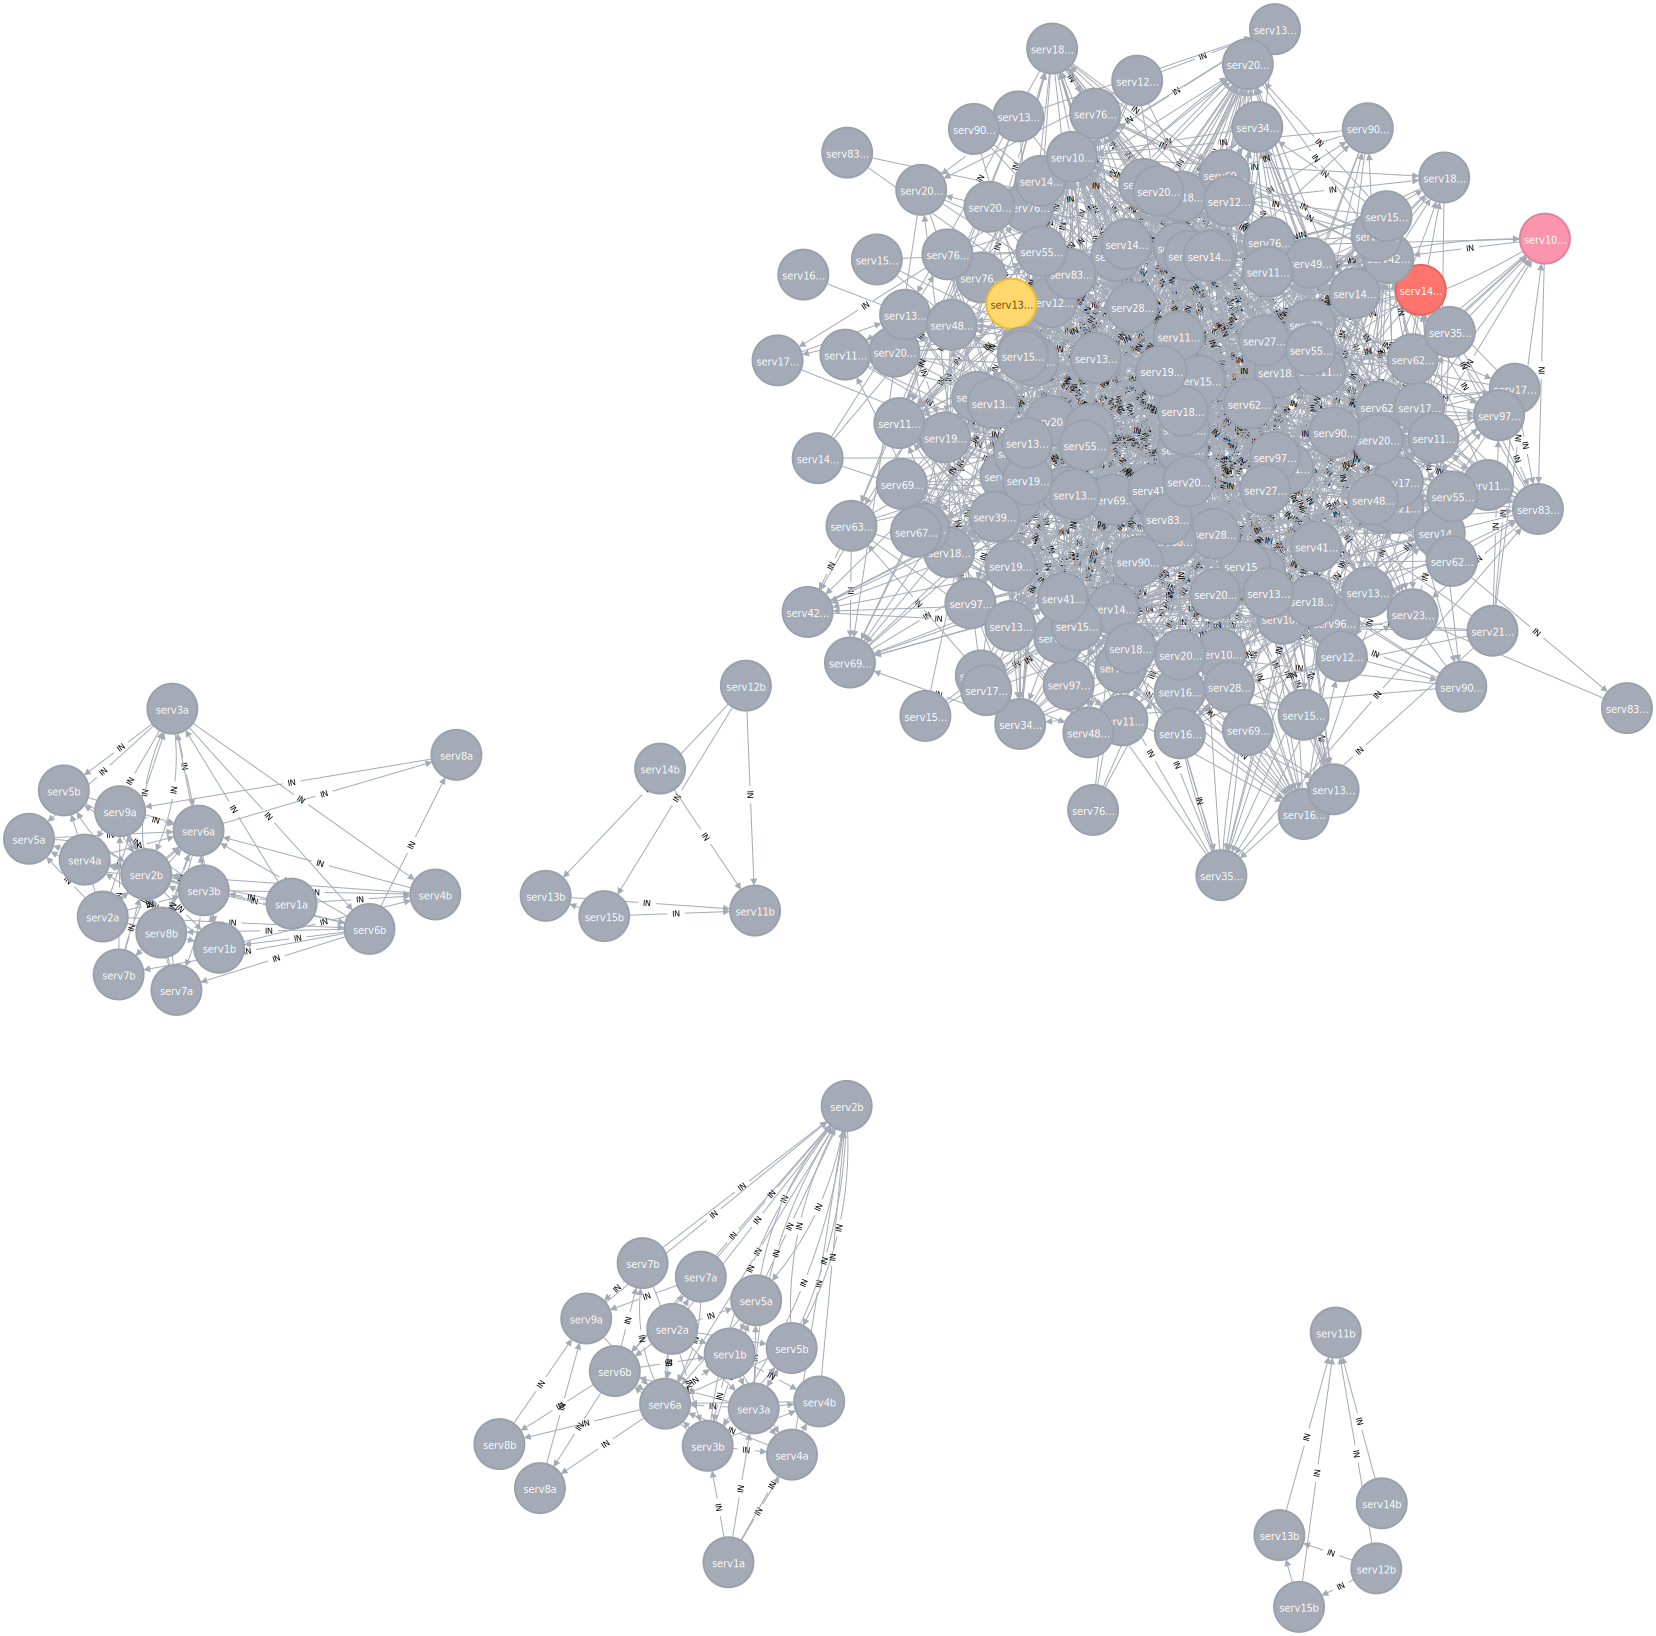
\includegraphics[width = 13cm, height = 10cm, scale = 0.5]{svg-before-reduce.pdf}
\centering
\caption{Graph database before reduction (WSC 2008 - 01)}
\label{fig:beforeReduction} 
\end{figure} 

\begin{figure}[H]
\includegraphics[scale = 0.6]{The-properties-of-Web-service-serv213889376.pdf}
\centering
\caption{The properties of Web service serv7231183 (WSC 2008 - 01)}
\label{fig:servProp} 
\end{figure} 

\section{Generate a Graph Database for a Given Task}
For each given task which is described by $\{inputs, outputs\}$, only a subset of services in a repository is related to that task. Therefore we created a graph database for each given task. This section presents an algorithm that generates a reduced graph for a given task, as shown in \emph{Algorithm 4}. \\

\begin{algorithm}[H]
 \SetKwInOut{Input}{Input}\SetKwInOut{Output}{Output}
 \SetKwFunction{connectNode}{connectNode}\SetKwFunction{findCands}{findCands}\SetKwFunction{removeDangling}{removeDangling}
 \LinesNumbered
 \SetNlSty{}{}{:}
  \Input{$GraphDatabase$}
 \Output{$ReducedGraphDatabase$}
 $i \leftarrow 0$\;
 $relatedNodes \leftarrow \{\}$\;
 \While{$i < |serviceNodes|$}{\label{buildingLine}
   $sNode \leftarrow serviceNodes[i]$\;
   \If {$hasRelationship(sNode, startNode) \wedge hasRelationship(sNode, endNode)$}{\label{buildingLine}
        $relatedNodes \leftarrow relatedNodes\cup \{sNode\}$\;
   }
   \If {$!fulfillInputs(sNode)$}{\label{buildingLine}
      $removeRelatedNodes(sNode)$\;
   }
   $i \leftarrow i+1$\;
  }
  \Return { $relatedNodes $\;}
 \caption{\footnotesize Reduce Graph Database.}
\label{generation}
\end{algorithm}
\setlength{\textfloatsep}{20pt}% Remove \textfloatsep

\par

Our algorithm first creates a start node \emph{S} and an end node \emph{E}. The start node \emph{S} contains the inputs of the task and the end node \emph{E}  contains the outputs of the task. Secondly, we insert these nodes into the database by creating new relationships between start node \emph{S} and all the nodes that use \emph{S}'s input. Similarly, we create relationships between end node \emph{E} and all the nodes that can output data to node \emph{E}. Lastly, we find all services that lie on a path between \emph{S} and \emph{E} and remove all services that are not a path. \emph{Algorithm 4} shows the process of reducing the original graph database by removing all nodes which do not lie on a path between \emph{S} and \emph{E}.

\begin{example}
\noindent
The following example illustrates the effectiveness of our proposed algorithm. Applying our graph database reduction algorithm (\emph{Algorithm 4}) to the graph database shown in Figure \ref{fig:inputOutputServs} leads to the new reduced graph database shown in Figure \ref{fig:reduced}. This new reduced graph database contains only Web services which are related to both task \emph{input} and task \emph{output}. Applying this procedure to the database chosen in this example reduces the number of Web services in the graph database from 158 to 61.
\end{example}

\begin{figure}[H]
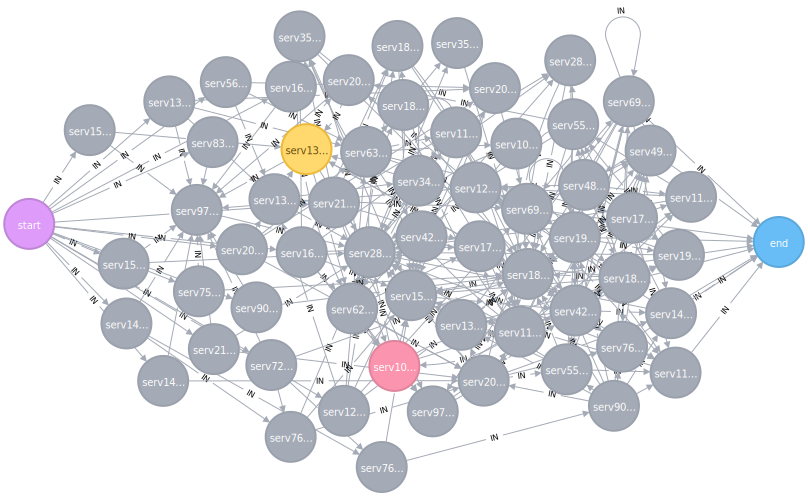
\includegraphics[width = 13cm, height = 10cm, scale = 0.5]{svg-reduced.pdf}
\centering
\caption{Reduced graph database (WSC2008-01)}
\label{fig:reduced} 
\end{figure} 

\section{Generating Web Service Compositions} \label{generatingComp}
Our reduced graph database algorithm allows us to retrieve all the Web service nodes related to a particular task. This section explains how we used related Web service nodes to generate Web service compositions in order to create an initial set of candidates.\par

\emph{Algorithm 5} is designed to create feasible compositions. It starts from the end node and searches internal nodes which are directly connected to the end node. Internal nodes are added into the composition list if they fulfill the input of the end node. Then the algorithm recursively goes through each node in the composition list and repeats the above steps until the size of the composition list is stable. This algorithm is also able to calculate the total response time for the creation of each composition,thus determining the total response time from task \emph{input} to task \emph{output}. This total  response time is then used to determine the quality of the solution, when we generate a \emph{QoS}-Aware service composition. \emph{Algorithm 5} calculates the response time during generation of the Web service composition by setting the duration property which reflects the time taken from End Node to Start Node. When adding node \emph{N} to the composition list, the algorithm first checks the \emph{druation} property of node \emph{N}. If \emph{N}'s duration property value is less than the sum of \emph{N}'s previous node  duration property value and  \emph{N}'s execution time ( \emph{N}'s \emph{QoS} time value), then the algorithm sets  \emph{N}'s duration property value to the sum of the  \emph{N}'s previous node duration property value and  \emph{N}'s execution time.\par

\begin{algorithm}[H]
 \SetKwInOut{Input}{Input}\SetKwInOut{Output}{Output}
 \SetKwFunction{connectNode}{connectNode}\SetKwFunction{findCands}{findCands}\SetKwFunction{removeDangling}{removeDangling}
 \LinesNumbered
 \SetNlSty{}{}{:}
   \Input{$endNode$, $relatedNodes$}
 \Output{$candidates$}
   $i \leftarrow 0$\;
   $relationships \leftarrow \{\}$\;
   $candidates \leftarrow \{\}$\; 
   \While{$i < |getIncomingRelationships(endNode)|$}{\label{buildingLine}
       $relationships \leftarrow relationships\cup \{tNode.getIncomingRelationships(endNode)[i]\}$\;
         $i \leftarrow i+1$\;
   }

   $fulfilledNodes \leftarrow fulfilledNodes \cup \{getNodesFulfillCurrentNode(rels)\}$\;
   \If {$| fulfilledNodes | > 0$}{\label{buildingLine}
        $candidates \leftarrow candidates\cup \{fulfilledNodes\}$\;
      $j \leftarrow 0$\;
      \While{$i < |candidates|$}{\label{buildingLine}
        $Recursively Call This Method Until The Size Of FulfillNodes Equals 0$\;
        $j \leftarrow i+1$\;
      }

   }
 \caption{\footnotesize Web services composition algorithm (initial populations).}
\label{generation}
\end{algorithm}
\setlength{\textfloatsep}{20pt}% Remove \textfloatsep

Two examples of Web service composition are shown in Figure \ref{fig:compEg1} and Figure \ref{fig:compEg2} to illustrate the application of our Web service composition algorithm (\emph{Algorithm 5}) to the reduced graph database we generated in Figure \ref{fig:reduced}. Both compositions show the relationship between task \emph{input} and task \emph{output}. For each node in the composition it is possible to click the Web service node \emph{S} to find the inputs of \emph{S} and also click the incoming edge of \emph{S} to find the input values related to the Web service which lies at the other end of the edge. \par
\begin{figure}[h]
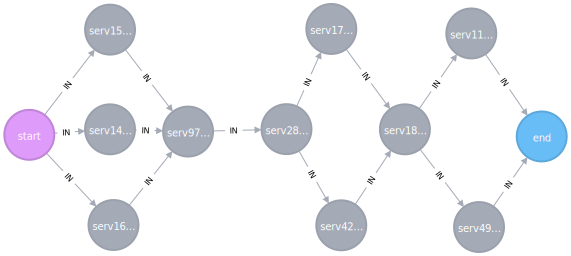
\includegraphics[width=11cm]{svg-composition1.pdf}
\centering
\caption{Web service composition 1 (dataset01, WSC2008)}
\label{fig:compEg1} 
\end{figure} 

\begin{figure}[h]
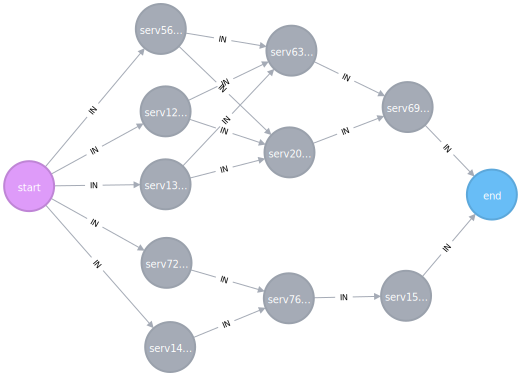
\includegraphics[width=11cm]{svg-composition2.pdf}
\centering
\caption{Web service composition 2 (dataset01, WSC2008)}
\label{fig:compEg2} 
\end{figure} 

\section{\emph{QoS}-Aware Service Composition}

In section \ref{generatingComp}, we proposed a Web service composition algorithm. The Web service composition algorithm we proposed uses a reduced number of Web services to search for service composition solutions using the smallest number of Web services possible.\par

The next step in our approach is to select a service composition for a set of solutions, which presents the best \emph{QoS} for a given task. There are many service compositions which can fulfill a given task. As we can see in section 1, to meet a user's non-functional requirements, we must aim to find a service composition that proves to have the best \emph{QoS}.\par

Algorithm 6 is designed to search for the solution with best \emph{QoS}. Using the set of initial population generated from \emph{Algorithm 5}, the algorithm goes through each and every service node invoked in the compositions. It then determines minimums and maximums of execution cost, response time, availability and reliability. Having found all minimums and maximums the next steps are to carry out normalization to restrict all values to the interval \emph{[0,1]}, and then to apply a fitness function, using normalized \emph{QoS} properties and user defined weights (see section \ref{fitnessFunction}), to each service composition. Lastly, the algorithm returns the service composition which has the best fitness value. \par

The following example shows a comparison of two compositions and uses data from Table \ref{tb:compExample}, which contains \emph{QoS} properties and fitness values of web service compositions. \\

\begin{example}
\noindent
EXAMPLE SHOWING THE COMPARISON OF TWO WEB SERVICE COMPOSITIONS
\setlength{\textfloatsep}{10pt}% Remove \textfloatsep
Composition 1 is shown in Figure \ref{fig:compEg1} and composition  2 is shown in Figure \ref{fig:compEg2}. To determine which is the better of the two compositions, we normalized the \emph{QoS} properties and used the fitness functions (section \ref{fitnessFunction}) of each service composition. Since we are only using two compositions in this example, the highest values on Availability and reliability, and the lowest values on Cost and Time will be equal or close to 1. We then set the weight for our fitness function to \emph{0.25}. The result in Table \ref{tb:compExample} shows that composition 2 (originally shown in \ref{fig:compEg2}) has the best fitness.  
\end{example}

% Please add the following required packages to your document preamble:
% \usepackage{multirow}
\begin{table}[H]
\centering
\caption{Comparison of two web service compositions}
\label{tb:compExample}
\scalebox{0.9}{
\begin{tabular}{|c|c|c|c|c|c|c|}
\hline
\multicolumn{2}{|c|}{\textbf{Compositions}}               & Cost   & Time     & Availability & Reliability & Fitness                 \\ \hline
\multirow{2}{*}{\textbf{1 (Figure \ref{fig:compEg1})}} & Non-normalized & 48.11  & 23427.83 & 1.60043E-5   & 0.00935     & \multirow{2}{*}{0.25}   \\ \cline{2-6}
                                         & Normalized     & 0.0    & 0.0      & 0.0          & 1.0         &                         \\ \hline
\multirow{2}{*}{\textbf{2 (Figure \ref{fig:compEg2})}} & Non-normalized & 44.18  & 12858.46 & 0.005        & 0.001408    & \multirow{2}{*}{0.7475} \\ \cline{2-6}
                                         & Normalized     & 0.9899 & 1.0      & 1.0          & 0.0         &                         \\ \hline
\end{tabular}
}
\end{table}

\begin{algorithm}[H]
 \SetKwInOut{Input}{Input}\SetKwInOut{Output}{Output}

 \SetKwFunction{connectNode}{connectNode}\SetKwFunction{findCands}{findCands}\SetKwFunction{removeDangling}{removeDangling}
 \LinesNumbered
 \SetNlSty{}{}{:}
  \Input{$InitialCompositions$, $weights$}
 \Output{$bestComposition$}
  $i \leftarrow 0$\;
 $BestComposition \leftarrow \{\}$\;
 $BestFintess \leftarrow 0$\; 
 $Map<composition, normalizedList> compWithNormalized \leftarrow \{\}$\;
 \While{$i < |InitialCompositions|$}{\label{buildingLine}
   $j \leftarrow 0$\;
     \While{$j < |InitialCompositions(i)|$}{\label{buildingLine}
      $find (maxC, minC, maxT, minT, maxA, minA, maxR, minR)$\;
      $j \leftarrow j+1$\;
  }
   $i \leftarrow i+1$\;
  }
  $i \leftarrow 0$\;
 \While{$i < |InitialCompositions|$}{\label{buildingLine}
   $j \leftarrow 0$\;
     \While{$j < |InitialCompositions(i)|$}{\label{buildingLine}
        $NormalizedList.add(normalize(Cost, Time, Availability, Availability));$
      $j \leftarrow j+1$\;
     }
     $compWithNormalized.getKey(composition) \leftarrow  NormalizedList;$

   $i \leftarrow i+1$\;
  }

  $i \leftarrow 0$\;
 \While{$i < |compWithNormalized|$}{\label{buildingLine}
    $fitnessValue = fitnessFunction(compWithNormalized(i), weights)$\;
      \If{$fitnessValue > BestFitness$}{
        $BestFitness \leftarrow  fitnessValue$\;
        $BestComposition \leftarrow  composition;$
        }
}
 \caption{\footnotesize \emph{QoS} aware Web services composition algorithm}
\label{generation}
\end{algorithm}
\chapter{Evaluation Design}\label{C:ed}
In this chapter we present our performance evaluation of our graph database based approach, by comparing it with an existing approach, namely, the GraphEvol approach presented in \cite{2}. In particular, we evaluated the effectiveness and efficiency of our approach by comparing the quality of composition solutions and the time taken to generate a Web service composition. 

\section{Datasets and Parameters} 
We evaluated the performance of our approach by testing it on a benchmark dataset, WSC2008 \cite{12} which contains service collections of varying sizes. To provide a comparison with the GraphEvol approach, we ran each task independently 30 times, for each run recording the best Web service composition, fitness value and execution time. For all tests we set the weights for an objective function to the same value as was used with the GraphEvol method, namely, a fixed weight of 0.25. The other parameters for GraphEvol were: a population of 200 candidates, a mutation probability of 0.05, and a crossover probability of 0.5. Individuals were chosen for breeding using tournament selection with a tournament size of 2 \cite{2}.\par

The test to compare the performance of the graph database approach and GraphEvol approach is conducted on a Macbook Pro Mid 2012 with a 2.9GHz dual-core Intel Core i7 processor, 8GB of 1600MHz DDR3 memory, a 1536 Mb Intel HD Graphics 4000 graphics card, a 128GB solid-state drive and the OS X EI Capitan operating system.

\section{Evaluation Results} 
In this section we present the results of our evaluation of our proposed algorithms. 

\subsection{Effectiveness of the Reducing Algorithm} 
To evaluate the effectiveness of our reducing graph database algorithm we applied it to all test cases contained of WSC2008 \cite{12}.  Table \ref{tb:reduce} shows the number of Web services for the original repositories and the number of Web service for the reduced graph database. For example, for WSC2008-02, there were 558 Web services in the original repository, but only 66 of them were related to the task input and task output. For task WSC2008-08, there were 8138 Web service in the original repository, but only 131 of them were related to the task input and output. Thus, the number of the Web services was greatly reduced when compared to the number in the original repositories, which greatly improved the execution time when generating the Web service composition.

\begin{table}[]
\centering
\caption{Comparison of the number of services in the original repositories and the reduced repositories}
\label{tb:reduce}
\scalebox{0.9}{

\begin{tabular}{|c|c|c|ll}
\cline{1-3}
Dataset WSC2008 & Original service repository & Reduced Service repository &  &  \\ \cline{1-3}
01              & 158                         & 61                         &  &  \\ \cline{1-3}
02              & 558                         & 66                         &  &  \\ \cline{1-3}
03              & 604                         & 105                        &  &  \\ \cline{1-3}
04              & 1041                        & 46                         &  &  \\ \cline{1-3}
05              & 1091                        & 102                        &  &  \\ \cline{1-3}
06              & 2198                        & 205                        &  &  \\ \cline{1-3}
07              & 4113                        & 195                        &  &  \\ \cline{1-3}
08              & 8119                        & 131                        &  &  \\ \cline{1-3}
\end{tabular}
}
\end{table}

\subsection{Correctness of the Web Service Composition} 
A composition correctness evaluation was carried out to check correctness of the Web service compositions. The correctness of the Web service composition was determined by checking that all the service node inputs are fulfilled by the output of their proceeding nodes in the graph database. We checked the correctness of all the service composition solutions produced by our algorithm. Our evaluation showed that all the solutions were correct. In this report, we show two composition solutions for Task 1 of WSC2008 with a repository of 158 services. The following examples show that for Task 1 the task and the service compositions produced by our approach (see Figure \ref{fig:c4compEg1} and Figure \ref{fig:c4compEg2}).\\

Task 1: \emph{WSC2008-01}\par
Task 1 inputs: \emph{[inst1926141668, inst395151449, inst1557679659]}\par
Task 1 outputs: \emph{[inst1913443608, inst664891780]}\\\par

\begin{figure}[h]
\includegraphics[width=11cm]{svg-chapter4-c1.pdf}
\centering
\caption{Web service composition 1 (Task1, WSC2008-01)}
\label{fig:c4compEg1} 
\end{figure} 
\begin{exmp}
In Figure \ref{fig:c4compEg1}, showing a example of Web service composition, the input of the Web service \emph{serv283321609} is \emph{I} = \emph{{ inst722854357, inst347634243, inst1881697469, inst746203847 }}. This matches the output  \emph{O} = \emph{{inst722854357, inst2092246857, inst1326239605, inst1881697469, inst1437249127, inst1519789560 }} of Web service  \emph{serv976005395}. This exact match occurs as \emph{inst722854357} and \emph{inst1881697469} are found in both Web service \emph{serv283321609} and Web service \emph{serv976005395}, while,  according to the taxonomy tree, \emph{inst1519789560} and \emph{inst1326239605} in \emph{O} are specializations of \emph{inst347634243} in \emph{I} and \emph{inst1437249127} in \emph{O} is a specialization of \emph{inst746203847} in \emph{I}.\par
\end{exmp}

\begin{figure}[h]
\includegraphics[width=11cm]{svg-chapter4-c2.pdf}
\centering
\caption{Web service composition 2 (Task1, WSC2008-01)}
\label{fig:c4compEg2} 
\end{figure} 

\begin{exmp}
In Figure \ref{fig:c4compEg2},  the input of the web service \emph{serv699915007} is \emph{I} = \emph{{inst102675811, inst1689375842, inst1716616603}}. This matches the output \emph{O$_1$} = \emph{{inst927259823,inst608977925 }} of Web service  \emph{serv2085282617} and the output \emph{O$_2$} = \emph{{inst885068313,inst1420249694,inst1488043421 }} of Web service  \emph{serv630482774}. As you can see there is no exact match between the outputs of services \emph{serv2085282617} and \emph{serv630482774}, and inputs of service \emph{serv699915007}, while, according to the taxonomy tree, \emph{inst1488043421} in \emph{O$_2$} is a specialization of inst102675811 in \emph{I}, \emph{inst927259823} in \emph{O$_1$} is a specialization of \emph{inst1689375842} in \emph{I} and  \emph{inst885068313} in \emph{O$_2$} is a specialization of \emph{inst1716616603} in \emph{I}.\par
\end{exmp}

Thus, the number of Web services involved in both examples is the same. Since we are only evaluating the correctness of the composition, we do not know whether the Web services composition is capable of performing tasks reliably or efficiently (i.e accounting for non-functional attributes). The next section presents the performance of our QoS-aware approach by comparing it with the GraphEvol approach.\par

\subsection{Evaluation Results for QoS-Aware Service Composition} 
Table \ref{tb:evalComp} shows a full evaluation comparing the performance of our approach and that of the  GraphEvol approach \cite{2}. Both approaches were run on the same machine (mentioned in Section 4.1) to conduct significant analyses. We ran each task independently, for each run recording the best Web service composition, the number of services involved, the fitness value and the execution time taken. Then we calculated the mean, standard deviation for the number of services involved, fitness values and execution times separately for each task. For each run, our approach generated \emph{50} candidates and the best solution from those candidates was chosen. For GraphEvol approach, the best candidate was generated from a population size of \emph{200}.\par

Table \ref{tb:evalComp} includes three columns for each approach. The \emph{number} column records the number of services involved in the best Web service composition.  The \emph{time} column records the average time, over 30 independent runs, which was taken to generate the best Web service composition. And the \emph{fitness} column records the average \emph{QoS} fitness value for the best Web service composition, calculated from 30 independent runs.

\begin{table}[h]
\centering
\caption{ Average results of the tests for QoS-aware service composition}
\label{tb:evalComp}
\scalebox{0.66}{
\begin{tabular}{|c|c|c|c|c|c|c|}
\hline
\textbf{Dataset} & \multicolumn{3}{c|}{\textbf{Graph Database Approach}} & \multicolumn{3}{c|}{\textbf{GraphEvol Approach}}  \\ \hline
\textbf{2008}    & \textbf{Number}   & \textbf{Time (ms)}   & \textbf{Fitness}   & \textbf{Number} & \textbf{Time (ms)} & \textbf{Fitness}    \\ \hline
1                & 10 \rlap{{$\pm$}}\hspace{0.4cm} 0.00             & 2197.90 \rlap{{$\pm$}}\hspace{0.4cm}329 \rlap{{$\downarrow$}}          & 0.521 \rlap{{$\pm$}}\hspace{0.4cm}0.169 \rlap{{$\downarrow$}}      & 10.63 \rlap{{$\pm$}}\hspace{0.4cm}2.17      & 4845.57 \rlap{{$\pm$}}\hspace{0.4cm}315.42     & 0.645 \rlap{{$\pm$}}\hspace{0.4cm}0.139                \\ \hline
2                & 5  \rlap{{$\pm$}}\hspace{0.4cm} 0.00               & 5347.13 \rlap{{$\pm$}}\hspace{0.4cm}880 \rlap{{$\uparrow$}}           & 0.48 \rlap{{$\pm$}}\hspace{0.4cm}0.152 \rlap{{$\downarrow$}}        & 5.87 \rlap{{$\pm$}}\hspace{0.4cm}2.12       & 3699.77 \rlap{{$\pm$}}\hspace{0.4cm}364.57     & 0.906 \rlap{{$\pm$}}\hspace{0.4cm}0.00                  \\ \hline
3                & 40 \rlap{{$\pm$}}\hspace{0.4cm} 0.00               & 10961.53 \rlap{{$\pm$}}\hspace{0.4cm}790 \rlap{{$\downarrow$}}         & 0.387 \rlap{{$\pm$}}\hspace{0.4cm}0.1 \rlap{{$\uparrow$}}         & 41.2 \rlap{{$\pm$}}\hspace{0.4cm}0.79       & 17221.53 \rlap{{$\pm$}}\hspace{0.4cm}764.85    & 0.176 \rlap{{$\pm$}}\hspace{0.4cm}0.045           \\ \hline
4                & 10 \rlap{{$\pm$}}\hspace{0.4cm} 0.00              & 3885.70 \rlap{{$\pm$}}\hspace{0.4cm}399 \rlap{{$\downarrow$}}          & 0.431 \rlap{{$\pm$}}\hspace{0.4cm}0.066 \rlap{{$\uparrow$}}       & 10.2 \rlap{{$\pm$}}\hspace{0.4cm}0.48       & 6076.7 \rlap{{$\pm$}}\hspace{0.4cm}281.58      & 0.305 \rlap{{$\pm$}}\hspace{0.4cm}0.066            \\ \hline
5                & 20 \rlap{{$\pm$}}\hspace{0.4cm} 0.00             & 4510.6 \rlap{{$\pm$}}\hspace{0.4cm}468 \rlap{{$\downarrow$}}           & 0.403 \rlap{{$\pm$}}\hspace{0.4cm}0.128\rlap{{$\uparrow$}}        & 22.13 \rlap{{$\pm$}}\hspace{0.4cm}2.59      & 10444.2 \rlap{{$\pm$}}\hspace{0.4cm}572.59     & 0.164 \rlap{{$\pm$}}\hspace{0.4cm}0.046            \\ \hline
6                & 40 \rlap{{$\pm$}}\hspace{0.4cm} 0.00              & 258503.33 \rlap{{$\pm$}}\hspace{0.4cm}42324 \rlap{{$\uparrow$}}       & 0.407 \rlap{{$\pm$}}\hspace{0.4cm}0.089 \rlap{{$\uparrow$}}       & 40.2 \rlap{{$\pm$}}\hspace{0.4cm}0.48       & 22183.53 \rlap{{$\pm$}}\hspace{0.4cm}1639      & 0.228 \rlap{{$\pm$}}\hspace{0.4cm}0.06           \\ \hline
7                & 20 \rlap{{$\pm$}}\hspace{0.4cm} 0.00              & 17839.77 \rlap{{$\pm$}}\hspace{0.4cm}763 \rlap{{$\downarrow$}}          & 0.457 \rlap{{$\pm$}}\hspace{0.4cm}0.097 \rlap{{$\uparrow$}}       & 23.13 \rlap{{$\pm$}}\hspace{0.4cm}7.33      & 20304.37 \rlap{{$\pm$}}\hspace{0.4cm}1257      & 0.316 \rlap{{$\pm$}}\hspace{0.4cm}0.039          \\ \hline
8                & 30 \rlap{{$\pm$}}\hspace{0.4cm} 0.00              & 53003.7 \rlap{{$\pm$}}\hspace{0.4cm}4465 \rlap{{$\uparrow$}}          & 0.468 \rlap{{$\pm$}}\hspace{0.4cm}0.091 \rlap{{$\uparrow$}}       & 32.47 \rlap{{$\pm$}}\hspace{0.4cm}3.86      & 18567.03 \rlap{{$\pm$}}\hspace{0.4cm}2055      & 0.315 \rlap{{$\pm$}}\hspace{0.4cm}0.028                \\ \hline
\end{tabular}
}
\end{table}

% \begin{table}[h]
% \centering
% \caption{ Average results of the tests for QoS-Aware service composition}
% \label{tb:evalComp}
% \scalebox{0.66}{
% \begin{tabular}{|c|c|c|c|c|c|c|c|c|}
% \hline
% \textbf{Dataset} & \multicolumn{3}{c|}{\textbf{Graph Database (Neo4j) Approach}} & \multicolumn{3}{c|}{\textbf{GraphEvol Approach}}        & \multicolumn{2}{c|}{\textbf{T-Test P value}} \\ \hline
% \textbf{2008}    & \textbf{Number}   & \textbf{Time (ms)}   & \textbf{Fitness}   & \textbf{Number} & \textbf{Time (ms)} & \textbf{Fitness} & \textbf{Fitness}       & \textbf{Time}       \\ \hline
% 1                & 10 \rlap{{$\pm$}}\hspace{0.4cm} 0.00             & 2197.90 \rlap{{$\pm$}}\hspace{0.4cm}329 \rlap{{$\downarrow$}}          & 0.521 \rlap{{$\pm$}}\hspace{0.4cm}0.169       & 10.63 \rlap{{$\pm$}}\hspace{0.4cm}2.17      & 4845.57 \rlap{{$\pm$}}\hspace{0.4cm}315.42     & 0.645 \rlap{{$\pm$}}\hspace{0.4cm}0.139      & 0.999                  & 6.96E-38            \\ \hline
% 2                & 5  \rlap{{$\pm$}}\hspace{0.4cm} 0.00               & 5347.13 \rlap{{$\pm$}}\hspace{0.4cm}880           & 0.48 \rlap{{$\pm$}}\hspace{0.4cm}0.152         & 5.87 \rlap{{$\pm$}}\hspace{0.4cm}2.12       & 3699.77 \rlap{{$\pm$}}\hspace{0.4cm}364.57     & 0.906 \rlap{{$\pm$}}\hspace{0.4cm}0.00       & 0.9999                 & 0.99999             \\ \hline
% 3                & 40 \rlap{{$\pm$}}\hspace{0.4cm} 0.00               & 10961.53 \rlap{{$\pm$}}\hspace{0.4cm}790 \rlap{{$\downarrow$}}         & 0.387 \rlap{{$\pm$}}\hspace{0.4cm}0.1 \rlap{{$\uparrow$}}         & 41.2 \rlap{{$\pm$}}\hspace{0.4cm}0.79       & 17221.53 \rlap{{$\pm$}}\hspace{0.4cm}764.85    & 0.176 \rlap{{$\pm$}}\hspace{0.4cm}0.045      & 2.38E-13               & 2.06E-37            \\ \hline
% 4                & 10 \rlap{{$\pm$}}\hspace{0.4cm} 0.00              & 3885.70 \rlap{{$\pm$}}\hspace{0.4cm}399 \rlap{{$\downarrow$}}          & 0.431 \rlap{{$\pm$}}\hspace{0.4cm}0.066 \rlap{{$\uparrow$}}       & 10.2 \rlap{{$\pm$}}\hspace{0.4cm}0.48       & 6076.7 \rlap{{$\pm$}}\hspace{0.4cm}281.58      & 0.305 \rlap{{$\pm$}}\hspace{0.4cm}0.066      & 5.58E-110              & 3.03E-30            \\ \hline
% 5                & 20 \rlap{{$\pm$}}\hspace{0.4cm} 0.00             & 4510.6 \rlap{{$\pm$}}\hspace{0.4cm}468 \rlap{{$\downarrow$}}           & 0.403 \rlap{{$\pm$}}\hspace{0.4cm}0.128\rlap{{$\uparrow$}}        & 22.13 \rlap{{$\pm$}}\hspace{0.4cm}2.59      & 10444.2 \rlap{{$\pm$}}\hspace{0.4cm}572.59     & 0.164 \rlap{{$\pm$}}\hspace{0.4cm}0.046      & 8.80E-12               & 1.95E-44            \\ \hline
% 6                & 40 \rlap{{$\pm$}}\hspace{0.4cm} 0.00              & 258503.33 \rlap{{$\pm$}}\hspace{0.4cm}42324      & 0.407 \rlap{{$\pm$}}\hspace{0.4cm}0.089 \rlap{{$\uparrow$}}       & 40.2 \rlap{{$\pm$}}\hspace{0.4cm}0.48       & 22183.53 \rlap{{$\pm$}}\hspace{0.4cm}1639      & 0.228 \rlap{{$\pm$}}\hspace{0.4cm}0.06       & 1.81E-12               & 1.0                   \\ \hline
% 7                & 20 \rlap{{$\pm$}}\hspace{0.4cm} 0.00              & 17839.77 \rlap{{$\pm$}}\hspace{0.4cm}763 \rlap{{$\downarrow$}}          & 0.457 \rlap{{$\pm$}}\hspace{0.4cm}0.097 \rlap{{$\uparrow$}}       & 23.13 \rlap{{$\pm$}}\hspace{0.4cm}7.33      & 20304.37 \rlap{{$\pm$}}\hspace{0.4cm}1257      & 0.316 \rlap{{$\pm$}}\hspace{0.4cm}0.039      & 3.83E-09               & 3.98E-12            \\ \hline
% 8                & 30 \rlap{{$\pm$}}\hspace{0.4cm} 0.00              & 53003.7 \rlap{{$\pm$}}\hspace{0.4cm}4465         & 0.468 \rlap{{$\pm$}}\hspace{0.4cm}0.091 \rlap{{$\uparrow$}}       & 32.47 \rlap{{$\pm$}}\hspace{0.4cm}3.86      & 18567.03 \rlap{{$\pm$}}\hspace{0.4cm}2055      & 0.315 \rlap{{$\pm$}}\hspace{0.4cm}0.028      & 1.44E-10               & 1.0                   \\ \hline
% \end{tabular}
% }
% \end{table}

\subsubsection{The number of the Web services involved} 

The results in Table \ref{tb:servSize} compare the number of Web services required for a composition using two approaches. The result (number of services invoked) with the {'}\emph{minimum number of Web services}{'} approach was equal to or very close to the result using the {'}\emph{non-minimum number of Web services}{'} approach. However, the fitness values were much higher with the {'}\emph{minimum number of Web services}{'} approach. A poor result occurred with Datasets \emph{1} and \emph{3}, and with Dataset \emph{3} the {'}\emph{non-minimum number of Web services}{'} approach took \emph{1138667.65} milliseconds (\emph{19} minutes) to generate a single service composition due to the huge search space involved, compared with \emph{10916.53} milliseconds (\emph{10.9} seconds) using the the {'}\emph{minimum number of Web services}{'} method. This was because when we restrict our approach to a minimum number of Web services, the search space is also restricted. The result was that when we added web service nodes into the service composition, whenever the number of the web services in the composition was greater than the minimum number of the Web services, our approach led to continual re-starting of the composition generation step in order to find a new composition.\par

So we decided to use the {'}\emph{minimum number of Web services}{'} method to generate Web service compositions in order to find the best candidates. The result was that the number of the services involved in our approach was less than or equal to the numbers of services when using the GraphEvol approach.\par

\subsubsection{Execution time to generate best QoS-Aware Web service composition} 
Our approach successfully generated a Web service composition for each task in eight datasets from WSC2008. For five tasks our approach was significantly better than the GraphEvol approach in terms of execution time. However, the composition generation time for the remaining three tasks was slower than when using the GraphEvol approach. This was especially true for Dataset \emph{6}, which took \emph{258503.33} milliseconds using our approach compared with \emph{22183.53} milliseconds using the GraphEvol approach.\par

The result we obtained when using our algorithm with Dataset \emph{6} occurred because Dataset \emph{6} required \emph{40} Web service nodes for the composition and the reduced graph database contained \emph{205} Web service nodes. So one of five nodes was involved in the composition leading to a large number of edges (relationships) between the Web service nodes, and the large number of service nodes and edges increased the search space, thus increasing the total execution time in generating a composition. But overall, our approach performed better than the GraphEvol approach and led to faster generation of web compositions.\par



\begin{table}[h]
\centering
\caption{ Graph Database: Average (30 independent runs) results}
\label{tb:servSize}
\scalebox{0.8}{
\begin{tabular}{|c|c|c|c|c|c|c|}
\hline
Dataset & \multicolumn{3}{c|}{Using minimum number of services} & \multicolumn{3}{c|}{Using non-minimum number of  services} \\ \hline
2008    & Number        & Time (ms)          & Fitness          & Number            & Time (ms)           & Fitness          \\ \hline
1       & 10 \rlap{{$\pm$}}\hspace{0.4cm} 0.00            & 2197.90 \rlap{{$\pm$}}\hspace{0.4cm} 329  \rlap{{$\uparrow$}}       & 0.52\rlap{{$\pm$}}\hspace{0.4cm}0.166        & 10 \rlap{{$\pm$}}\hspace{0.4cm} 0.00               & 1047.06 \rlap{{$\pm$}}\hspace{0.4cm} 367          & 0.53 \rlap{{$\pm$}}\hspace{0.4cm} 0.174        \\ \hline
2       & 5 \rlap{{$\pm$}}\hspace{0.4cm} 0.00           & 5347.13\rlap{{$\pm$}}\hspace{0.4cm}880  \rlap{{$\uparrow$}}      & 0.54\rlap{{$\pm$}}\hspace{0.4cm}0.103        & 5 \rlap{{$\pm$}}\hspace{0.4cm} 0.00                & 3699.77\rlap{{$\pm$}}\hspace{0.4cm}364.57       & 0.546\rlap{{$\pm$}}\hspace{0.4cm}0.179       \\ \hline
4       & 10 \rlap{{$\pm$}}\hspace{0.4cm} 0.00           & 3885.70\rlap{{$\pm$}}\hspace{0.4cm}399  \rlap{{$\downarrow$}}       & 0.388\rlap{{$\pm$}}\hspace{0.4cm}0.08       & 10 \rlap{{$\pm$}}\hspace{0.4cm} 0.00               & 6076.7\rlap{{$\pm$}}\hspace{0.4cm}281.58        & 0.26\rlap{{$\pm$}}\hspace{0.4cm}0.028        \\ \hline
3       & 40 \rlap{{$\pm$}}\hspace{0.4cm} 0.00           & 10961.53\rlap{{$\pm$}}\hspace{0.4cm}790 \rlap{{$\downarrow$}}        & 0.387\rlap{{$\pm$}}\hspace{0.4cm}0.1        & 40 \rlap{{$\pm$}}\hspace{0.4cm} 0.00                 & 1138667.65 \rlap{{$\pm$}}\hspace{0.4cm}83582.58                 & 0.211\rlap{{$\pm$}}\hspace{0.4cm}0.068               \\ \hline
5       & 20 \rlap{{$\pm$}}\hspace{0.4cm} 0.00           & 4510.6\rlap{{$\pm$}}\hspace{0.4cm}468  \rlap{{$\downarrow$}}       & 0.398\rlap{{$\pm$}}\hspace{0.4cm}0.121      & 20 \rlap{{$\pm$}}\hspace{0.4cm} 0.00               & 10444.2\rlap{{$\pm$}}\hspace{0.4cm}572.59       & 0.227\rlap{{$\pm$}}\hspace{0.4cm}0.065       \\ \hline
6       & 40 \rlap{{$\pm$}}\hspace{0.4cm} 0.00           & 258503.33\rlap{{$\pm$}}\hspace{0.4cm}42324 \rlap{{$\uparrow$}}      & 0.354\rlap{{$\pm$}}\hspace{0.4cm}0.103       & 42.067\rlap{{$\pm$}}\hspace{0.4cm}1.29        & 22183.53\rlap{{$\pm$}}\hspace{0.4cm}1639         & 0.206\rlap{{$\pm$}}\hspace{0.4cm}0.086       \\ \hline
7       & 20 \rlap{{$\pm$}}\hspace{0.4cm} 0.00           & 17839.77\rlap{{$\pm$}}\hspace{0.4cm}763  \rlap{{$\downarrow$}}     & 0.411\rlap{{$\pm$}}\hspace{0.4cm}0.076      & 20 \rlap{{$\pm$}}\hspace{0.4cm} 0.00               & 20304.37\rlap{{$\pm$}}\hspace{0.4cm}1257         & 0.317\rlap{{$\pm$}}\hspace{0.4cm}0.085       \\ \hline
8       & 30 \rlap{{$\pm$}}\hspace{0.4cm} 0.00           & 53003.7\rlap{{$\pm$}}\hspace{0.4cm}4465  \rlap{{$\downarrow$}}     & 0.438\rlap{{$\pm$}}\hspace{0.4cm}0.012      & 33.67\rlap{{$\pm$}}\hspace{0.4cm}2.29         & 284831.37\rlap{{$\pm$}}\hspace{0.4cm}2125         & 0.358\rlap{{$\pm$}}\hspace{0.4cm}0.052       \\ \hline
\end{tabular}
}
\end{table}

\subsubsection{Hypothesis test using two fitness value sets for each approach} 

We used a two-sample t-test to check if the fitness values and execution times for our approach were better than the fitness values and execution times for the GraphEvol approach at the \emph{0.05} significance level. In Table \ref{tb:evalComp}, it is clear that the P-values from datasets \emph{03} to \emph{08} are smaller than the significance level \emph{0.05} for the fitness values set and Datasets \emph{1, 3, 4, 5} and \emph{7} are less than the significance level \emph{0.05} for the execution times set, as indicated by the upward and downward pointing arrows. This means there is considerable evidence that the sets of fitness values and execution times for GraphEvol approach are lower than for our approach. In other words, the best solutions in our approach are significantly superior to the best solutions produced by the GraphEvol approach for 6 out of 8 tasks. For execution time, our approach are faster than GraphEvol for 5 out of 8 tasks and only with Dataset \emph{2, 6} and \emph{8} were our execution time sets poorer than with the GraphEvol approach. In summary however, our approach successfully produced a better result overall, than the GraphEvol approach, in most test cases using the benchmark dataset.\par

\subsection{Summary}
This chapter we evaluate  the performance of our proposed graph database-based approach with an existing GP-based approach by comparing with an existing GP-based approach known as GraphEvol, which is presented in \cite{2}. From our evaluation results, we can conclude that our approach is efficient and effective in generating service composition solutions. It can generate near-optimal QoS-aware composition solutions in a shorter time than the GraphEvol approach.
\chapter{Conclusion and Future work}\label{C:conc}

This project proposed graph database-based approach to QoS-aware service composition. To do that we have proposed a model of service repository, so that information of services and relationships between services can be stored in graph databases. We have also proposed a QoS-aware service composition approach based on graph database.\par

We have tested this approach with all the service composition tasks from several collections of common benchmark test cases. We manually checked the correctness of all the inputs of service nodes in the web service composition for all the datasets in the WSC2008. Our composition correctness evaluation shows our approach is able to produce correct representations of service compositions.\par

We then extended our approach to QoS-aware web service compositions by considering additional QoS requirements. In order to compare the performance of our approach with the GraphEvol approach we used the following four QoS properties: availability, reliability, execution cost and execution duration. These QoS properties were then combined into a single fitness value for each composition. Finding the best web service composition was then possible using the fitness values of individual candidate web compositions we generated.\par

The results of our evaluation of this approach show that our algorithm can compute optimised solutions, and provides good performance comparing with an existing approach. With our approach, Web service nodes and edges (relationships) are stored in the Graph database permanently, and do not need to be re-created for each task. On the other hand, the problem of GraphEvol approach that only stores this information in memory rather than in permanent storage, and must constantly re-create relationships. This requires additional resources and leads to a longer processing time. GraphEvol also presents the additional challenge of maintaining the web service repository and the associated taxonomy tree, because of the overly complicated format used for storing data structures.\par

In this report, our approach used a reduced graph database that shrinks the search space for given task, thus improving its performance. In the future, we would like to investigate the generation of a QoS-aware web service composition using the original database, which does not decrease the performance of the solution. \par

Our approach did not save the task-related services for reuse in the future. Our future work will focus on saving all the task related services in local storage. With each task, if it is similar to a task already saved in local storage, we would reuse those saved task-related services instead of generating a task related reduced graph database from our original graph database. \par

We modelled only the service repository when developing our approach, which requires loading taxonomy.xml file from local storage. This method means it is impossible to modify the taxonomy file because of the format of the file. Moreover, whenever the taxonomy file changes, Web service graph database also needs to be updated for consistency.  Our future work on solving this shortcoming would focus on creating a graph database for taxonomy repository and trying to link all the taxonomy nodes with services' inputs and outputs. Thus every time taxonomy nodes were modified, service nodes would be automatically updated since they were interconnected. \par



%%%%%%%%%%%%%%%%%%%%%%%%%%%%%%%%%%%%%%%%%%%%%%%%%%%%%%%

\backmatter

%%%%%%%%%%%%%%%%%%%%%%%%%%%%%%%%%%%%%%%%%%%%%%%%%%%%%%%


%\bibliographystyle{ieeetr}
%\renewcommand\bibname{Bibliography} 
\bibliographystyle{acm}
\bibliography{sample}


\end{document}
